\documentclass[aspectratio=169,11pt]{beamer}

%% ── Theme ───────────────────────────────────────────────────────────────────
\usetheme{Madrid}
\usecolortheme{seahorse}
\setbeamertemplate{navigation symbols}{}
\setbeamertemplate{footline}[frame number]

%% ── Packages ────────────────────────────────────────────────────────────────
\usepackage[utf8]{inputenc}
\usepackage[vietnamese]{babel}
\usepackage{booktabs}
\usepackage{colortbl}
\usepackage{graphicx}
\usepackage{tikz}
\usetikzlibrary{arrows.meta, positioning, shapes.geometric}
\usepackage{amsmath,amssymb}
\usepackage{xcolor}
\usepackage{multirow}
\usepackage{pifont}  % \ding{51}=checkmark, \ding{55}=cross
\graphicspath{{figures/}}

%% ── Colors ──────────────────────────────────────────────────────────────────
\definecolor{primary}{RGB}{25,118,210}
\definecolor{success}{RGB}{46,125,50}
\definecolor{warning}{RGB}{230,81,0}
\definecolor{danger}{RGB}{183,28,28}
\definecolor{gancolor}{RGB}{156,39,176}
\definecolor{detcolor}{RGB}{33,150,243}
\definecolor{rowblue}{RGB}{227,242,253}
\definecolor{rowred}{RGB}{255,235,238}
\definecolor{rowgreen}{RGB}{232,245,233}
\definecolor{rowyellow}{RGB}{255,248,225}

\setbeamercolor{frametitle}{bg=primary,fg=white}
\setbeamercolor{title}{fg=primary}
\setbeamercolor{block title}{bg=primary,fg=white}
\setbeamercolor{block title alerted}{bg=danger,fg=white}
\setbeamercolor{block title example}{bg=success,fg=white}

\newcommand{\YES}{\textcolor{success}{\ding{51}}}
\newcommand{\NO}{\textcolor{danger}{\ding{55}}}

%% ── Metadata ────────────────────────────────────────────────────────────────
\title[GAN -- Sinh mẫu thử DDoS]
      {\textbf{Dùng GAN để phát sinh mẫu thử DDoS}}

\author[Nhóm 3 SV]{%
  \small
  \begin{tabular}{ll}
    1. Trần Đức Anh       & \textnormal{MHV: 250101005} \\
    2. Huỳnh Ngọc Hưng    & \textnormal{MHV: 250101027} \\
    3. Trần Thanh Dũng    & \textnormal{MHV: 250201053} \\
  \end{tabular}\\[4pt]
  \textnormal{\small\textit{Giảng viên hướng dẫn:} \textbf{PGS.TS. Nguyễn Tấn Cầm}}
}

\institute[]{}

\date{\today}

%% ─────────────────────────────────────────────────────────────────────────────
\begin{document}

%% ── TITLE ────────────────────────────────────────────────────────────────────
\begin{frame}
  \titlepage
\end{frame}

%% ── OUTLINE ──────────────────────────────────────────────────────────────────
\begin{frame}{Nội dung báo cáo}
  \tableofcontents
\end{frame}

%% =============================================================================
\section{1. Giới thiệu}
%% =============================================================================

\begin{frame}{Bối cảnh \& Động lực}
  \begin{columns}[T]
    \begin{column}{0.50\textwidth}
      \begin{alertblock}{Vấn đề}
        \begin{itemize}\setlength\itemsep{4pt}
          \item DDoS attacks ngày càng tinh vi
          \item IDS dựa ML cần \textbf{dữ liệu huấn luyện đa dạng}
          \item Dữ liệu DDoS thực: khó thu thập, mất cân bằng
        \end{itemize}
      \end{alertblock}
      \vspace{6pt}
      \begin{block}{Câu hỏi nghiên cứu}
        Liệu GAN có thể sinh ra fake DDoS traffic \textbf{đủ thực} để:
        \begin{enumerate}\setlength\itemsep{3pt}
          \item[\textbf{A.}] Test \& cải thiện IDS?
          \item[\textbf{B.}] Bypass detector hiện tại?
        \end{enumerate}
      \end{block}
    \end{column}
    \begin{column}{0.47\textwidth}
      \begin{exampleblock}{Đóng góp chính}
        \begin{enumerate}\setlength\itemsep{4pt}
          \item \textbf{Hướng A}: Pure WGAN sinh mẫu DDoS realistic
          \item \textbf{Hướng B}: Arms race GAN $\Leftrightarrow$ Detector (2 rounds)
          \item Đề xuất \textbf{Validity Score} -- metric mới đánh giá tính realistic
          \item SHAP explainability phân tích feature importance
        \end{enumerate}
      \end{exampleblock}
    \end{column}
  \end{columns}
\end{frame}

\begin{frame}{Dataset: CIC-DDoS2019}
  \begin{columns}[T]
    \begin{column}{0.48\textwidth}
      \begin{block}{Tổng quan}
        \small
        \begin{tabular}{ll}
          Nguồn & Canadian Institute for Cybersecurity \\
          \# Features & 80 (sau preprocessing) \\
          Train set & 68,380 samples \\
          Test set & 14,653 samples/class \\
        \end{tabular}
      \end{block}
      \vspace{2pt}
      \begin{block}{Phân loại features (novel)}
        \footnotesize
        \begin{itemize}\setlength\itemsep{2pt}
          \item \textcolor{danger}{\textbf{16 Functional:}} Protocol, Flag counts, Header Length, Flow Duration\\
          \textit{$\to$ Định nghĩa bản chất DDoS}
          \item \textcolor{detcolor}{\textbf{64 Non-functional:}} Packet stats, IAT, Byte counts\\
          \textit{$\to$ Biến đổi được mà không mất DDoS behavior}
        \end{itemize}
      \end{block}
    \end{column}
    \begin{column}{0.48\textwidth}
      \begin{exampleblock}{Ví dụ phân loại features}
        \footnotesize
        \begin{tabular}{lp{3cm}}
          \toprule
          \textbf{Loại} & \textbf{Feature} \\
          \midrule
          \textcolor{danger}{Functional} & SYN Flag Count \\
          \textcolor{danger}{Functional} & Protocol \\
          \textcolor{danger}{Functional} & Fwd Header Length \\
          \textcolor{danger}{Functional} & Flow Duration \\
          \midrule
          \textcolor{detcolor}{Non-functional} & Flow Bytes/s \\
          \textcolor{detcolor}{Non-functional} & Packet Length Mean \\
          \textcolor{detcolor}{Non-functional} & Flow IAT Std \\
          \bottomrule
        \end{tabular}
      \end{exampleblock}
    \end{column}
  \end{columns}
\end{frame}

%% =============================================================================
\section{2. Phương pháp đề xuất}
%% =============================================================================

\begin{frame}{Kiến trúc: WGAN-GP + MLP Detector}
  \begin{columns}[T]
    \begin{column}{0.50\textwidth}
      \begin{block}{Generator (G)}
        \footnotesize
        \begin{itemize}\setlength\itemsep{1pt}
          \item Input: $z \sim \mathcal{N}(0, I_{64})$
          \item Layers: $64 \to 128 \to 256 \to 256 \to 128 \to 80$
          \item Output: Fake DDoS sample (80 features)
        \end{itemize}
      \end{block}
      \vspace{2pt}
      \begin{block}{Critic (C) -- Wasserstein}
        \footnotesize
        \begin{itemize}\setlength\itemsep{1pt}
          \item Layers: $80 \to 256 \to 128 \to 64 \to 1$
          \item Loss: Wasserstein + Gradient Penalty ($\lambda_{GP}{=}10$)
        \end{itemize}
      \end{block}
      \vspace{2pt}
      \begin{block}{MLP Detector}
        \footnotesize
        \begin{itemize}\setlength\itemsep{1pt}
          \item Layers: $80 \to 256 \to 128 \to 64 \to 1$
          \item Activation: ReLU + Sigmoid, Dropout 0.3
        \end{itemize}
      \end{block}
    \end{column}
    \begin{column}{0.48\textwidth}
      \begin{alertblock}{Loss Function Generator}\vspace{-2pt}
        \textbf{Phase A:}\hspace{4pt}
        $\mathcal{L}_G = -\mathbb{E}[C(G(z))] + \lambda_c \mathcal{L}_{con}$
        \vspace{2pt}

        \textbf{Phase B:}\vspace{-8pt}
        \begin{align*}
          \mathcal{L}_G = &-\mathbb{E}[C(G(z))] + \lambda_{adv}\,\mathrm{BCE}\\
                         &+ \lambda_c\,\mathrm{MSE}(G(z)[F], \mu_F)
        \end{align*}
        \vspace{-12pt}

        \scriptsize
        $F$: functional features, $\mu_F$: mean real DDoS\\
        $\lambda_{adv}{=}1.0$, $\lambda_c{=}5.0$
      \end{alertblock}
    \end{column}
  \end{columns}
\end{frame}

\begin{frame}{Pipeline tổng thể}
  \centering
  \begin{tikzpicture}[
    node distance=0.6cm and 1.8cm,
    box/.style={draw, rounded corners=4pt, minimum width=2.8cm,
                minimum height=0.65cm, font=\small, align=center, fill=white},
    arrow/.style={-Stealth, thick},
    label/.style={font=\scriptsize, align=center}
  ]
    %% Row 1: Data + Phase A
    \node[box, fill=gray!15] (data) {CIC-DDoS2019};
    \node[box, fill=gancolor!25, draw=gancolor, below=0.7cm of data] (ga)
      {WGAN-GP\\Pure (Round 0)};
    \node[box, fill=gancolor!15, draw=gancolor, below=0.6cm of ga] (fake0)
      {Fake DDoS\\(Realistic)};

    %% Phase B nodes
    \node[box, fill=detcolor!25, draw=detcolor, right=2.5cm of data] (d1)
      {Detector v1\\(MLP Baseline)};
    \node[box, fill=gancolor!25, draw=gancolor, below=0.7cm of d1] (gb)
      {WGAN-GP\\Adversarial R1};
    \node[box, fill=detcolor!25, draw=detcolor, right=1.8cm of d1] (d2)
      {Detector v2\\(Adv. Training)};
    \node[box, fill=gancolor!25, draw=gancolor, below=0.7cm of d2] (gc)
      {WGAN-GP\\Adversarial R2};

    %% Arrows Phase A
    \draw[arrow, gancolor] (data) -- node[left, label]{} (ga);
    \draw[arrow, gancolor] (ga)   -- node[right, label]{Round 0} (fake0);

    %% Arrows Phase B
    \draw[arrow, detcolor] (data) -- (d1);
    \draw[arrow]           (d1)   -- node[left, label]{attack} (gb);
    \draw[arrow, gancolor] (gb.east) to[bend left=20]
                           node[below, label]{adv. train} (d2.south);
    \draw[arrow, detcolor] (d1)   -- node[above, label]{Phase 4} (d2);
    \draw[arrow]           (d2)   -- node[right, label]{attack R2} (gc);

    %% Phase labels
    \node[above=0.1cm of ga, font=\tiny\bfseries, gancolor] {Huong A};
    \node[above=0.1cm of d1, font=\tiny\bfseries, detcolor] {Huong B};
  \end{tikzpicture}
\end{frame}

%% =============================================================================
\section{3. Hướng A}
%% =============================================================================

\begin{frame}{Hướng A: Validity Score -- Metric mới đề xuất}
  \begin{columns}[T]
    \begin{column}{0.50\textwidth}
      \begin{block}{Định nghĩa Validity Score}
        \% fake samples có \textbf{tất cả} functional features trong valid range của real DDoS:
        \[
          V = \frac{1}{N}\sum_{i=1}^{N} \prod_{f \in F} \mathbf{1}[x_i^f \in [lo_f, hi_f]]
        \]
        Valid range: $[P_1, P_{99}]$ của real DDoS traffic
      \end{block}
      \vspace{6pt}
      \begin{alertblock}{Kết quả tổng thể}
        \centering \large
        \textbf{Overall Validity = 0\%}\\
        \small (AND condition: 11 features có valid range\\
        cực hẹp sau normalization)
      \end{alertblock}
    \end{column}
    \begin{column}{0.47\textwidth}
      \begin{exampleblock}{Per-feature Validity ($\lambda_c = 5.0$, Round 0)}
        \footnotesize
        \begin{tabular}{lc}
          \toprule
          \textbf{Feature} & \textbf{Validity} \\
          \midrule
          Flow Duration     & \textcolor{success}{\textbf{100.0\%}} \\
          ACK Flag Count    & \textcolor{success}{\textbf{99.9\%}}  \\
          Fwd URG Flags     & \textcolor{success}{\textbf{99.9\%}}  \\
          Bwd PSH Flags     & \textcolor{success}{\textbf{99.9\%}}  \\
          URG Flag Count    & \textcolor{success}{\textbf{99.7\%}}  \\
          \midrule
          Protocol          & \textcolor{danger}{0.0\%} \\
          SYN Flag Count    & \textcolor{danger}{0.0\%} \\
          Fwd Header Length & \textcolor{danger}{0.0\%} \\
          ... (8 others)    & \textcolor{danger}{0.0\%} \\
          \bottomrule
        \end{tabular}
      \end{exampleblock}
    \end{column}
  \end{columns}
\end{frame}

%% =============================================================================
\section{4. Hướng B}
%% =============================================================================

\begin{frame}{Hướng B: AUC cao -- Ý nghĩa vs F1=0}
  \begin{columns}[T]
    \begin{column}{0.50\textwidth}
      \begin{alertblock}{Hiện tượng thú vị}
        Round 2: \textbf{F1 = 0.0000} nhưng \textbf{AUC = 0.9888}
      \end{alertblock}
      \vspace{6pt}
      \begin{block}{Giải thích}
        \begin{itemize}\setlength\itemsep{4pt}
          \item AUC đo \textit{ranking}: detector vẫn gán xác suất DDoS cao hơn cho real DDoS so với fake
          \item Nhưng \textbf{tất cả fake samples} có $P < 0.5$ $\to$ phân loại là BENIGN
          \item GAN không cần tạo fake "giống real", chỉ cần \textbf{đẩy samples vào vùng BENIGN} của feature space
        \end{itemize}
      \end{block}
    \end{column}
    \begin{column}{0.47\textwidth}
      \begin{exampleblock}{Evasion Strategy}
        \centering
        \begin{tikzpicture}[scale=0.85]
          \draw[thick] (0,0) rectangle (4,3);
          \fill[success!20] (0,0) rectangle (4,1.2);
          \fill[danger!20]  (0,1.2) rectangle (4,3);
          \draw[dashed, thick] (0,1.2) -- (4,1.2)
            node[right, font=\tiny]{threshold=0.5};
          \node[font=\tiny, danger] at (2,2.2) {Real DDoS (P$>$0.5)};
          \node[font=\tiny, success] at (2,0.6) {BENIGN region};
          % Fake samples dots
          \foreach \x/\y in {0.5/0.3,1.2/0.5,2.0/0.4,2.8/0.6,3.5/0.3}
            \fill[gancolor] (\x,\y) circle (3pt);
          \node[font=\tiny, gancolor] at (2,-0.25)
            {Fake DDoS (P$<$0.5) $\leftarrow$ GAN pushes here};
        \end{tikzpicture}
      \end{exampleblock}
    \end{column}
  \end{columns}
\end{frame}

%% =============================================================================
\section{5. Thực nghiệm}
%% =============================================================================

\begin{frame}{Hướng A: Validity Heatmap -- Per-feature $\times$ Round}
  \begin{center}
    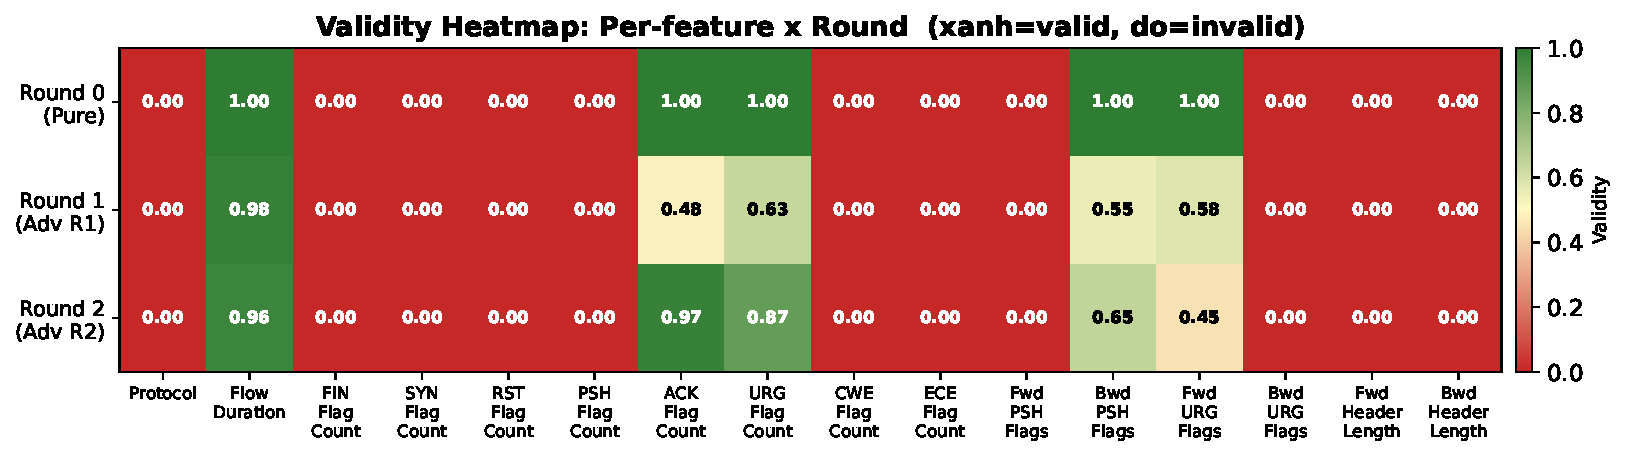
\includegraphics[width=0.97\textwidth,height=0.60\textheight,keepaspectratio]{fig_validity_heatmap}
  \end{center}
  \vspace{-4pt}
  \begin{columns}[T]
    \begin{column}{0.50\textwidth}
      \begin{alertblock}{\small Tại sao 11 features = 0\%?}\vspace{-2pt}
        \small Valid range sau normalization cực hẹp ($\min{\approx}\max$) -- GAN continuous float không thể rơi vào.\\
        \textit{Không phải lỗi GAN mà là đặc tính data.}
      \end{alertblock}
    \end{column}
    \begin{column}{0.47\textwidth}
      \begin{exampleblock}{\small Key finding + Hướng cải thiện}\vspace{-2pt}
        \small Round 0 giống real nhất (KL=1.49 vs 1.61 Adv).\\
        Fix: Post-processing snap về mode + Conditional GAN.
      \end{exampleblock}
    \end{column}
  \end{columns}
\end{frame}

\begin{frame}{Hướng A: Phân phối các features --- Real vs Fake DDoS}
  \begin{center}
    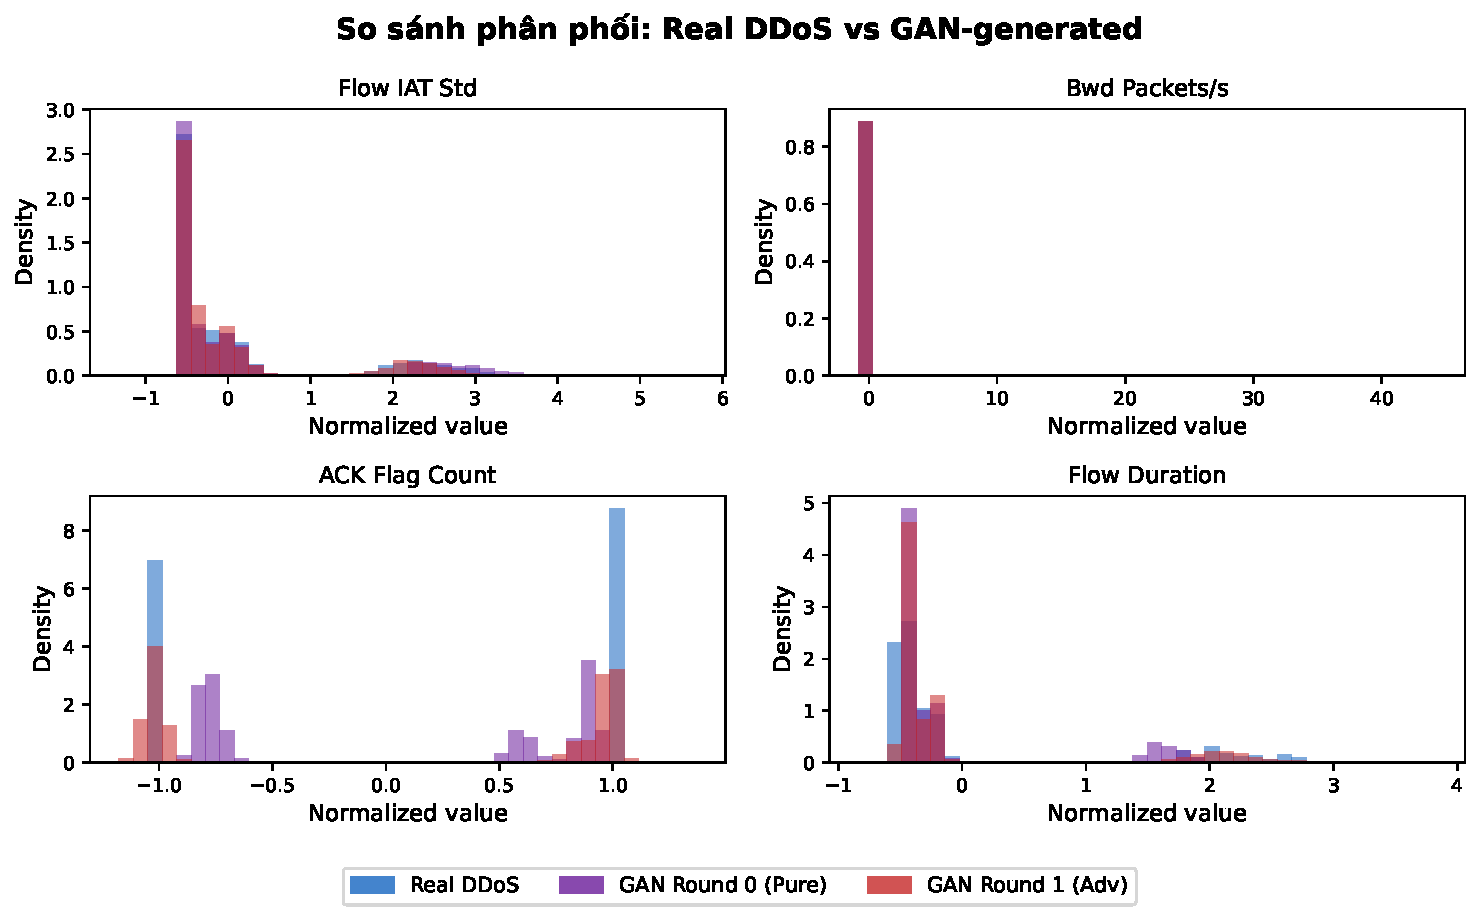
\includegraphics[width=0.95\textwidth,height=0.74\textheight,keepaspectratio]{fig_distribution}
  \end{center}
  \vspace{-4pt}
  \centering\footnotesize
  Pure GAN (tím) tiệm cận Real DDoS (xanh) hơn Adversarial GAN (đỏ)
\end{frame}

\begin{frame}{Hướng A: Per-feature Validity --- So sánh 3 round}
  \begin{center}
    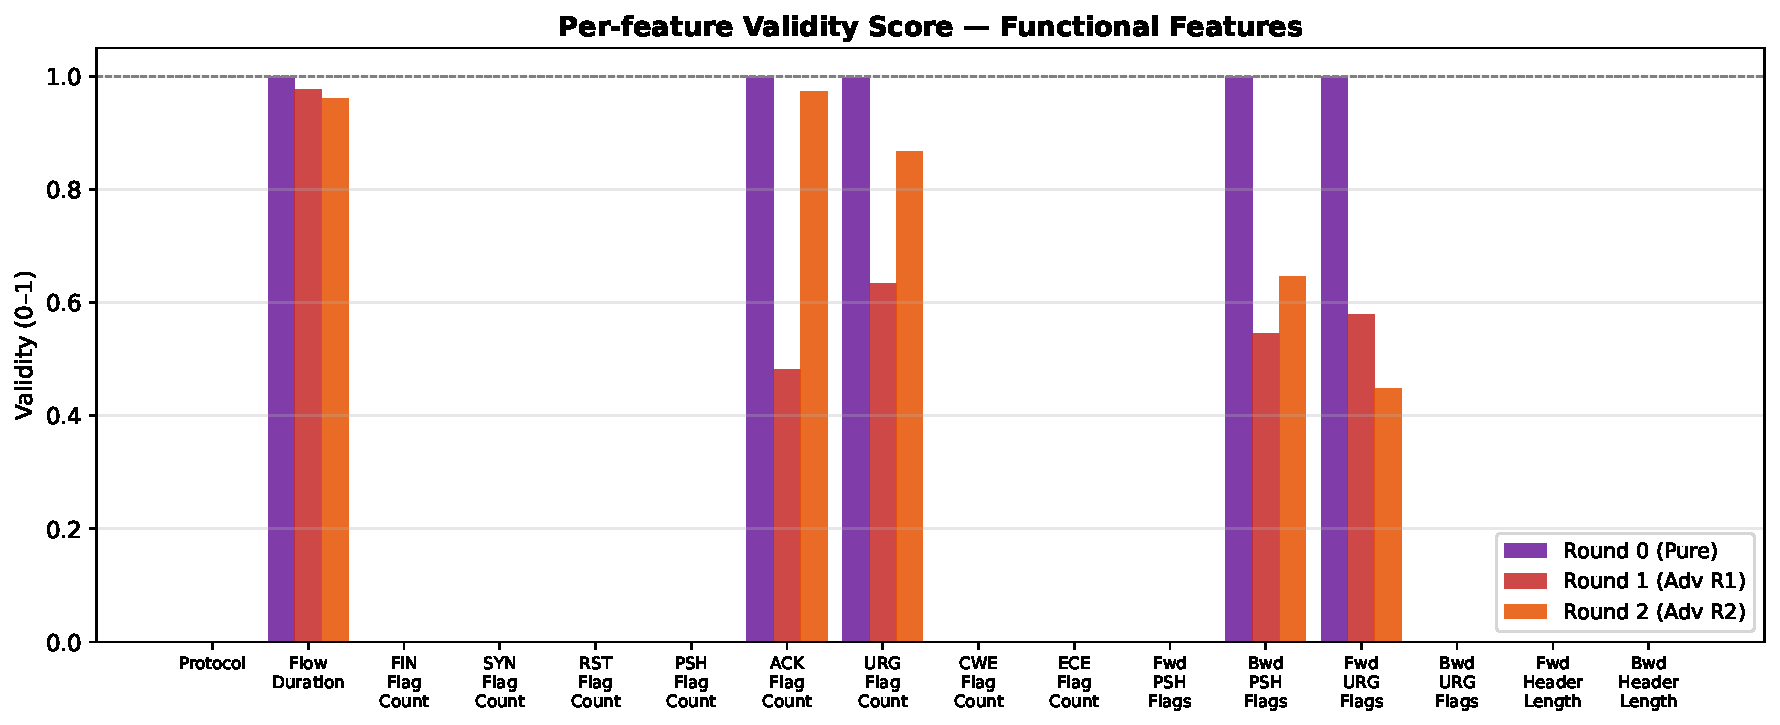
\includegraphics[width=0.97\textwidth,height=0.76\textheight,keepaspectratio]{fig_validity}
  \end{center}
  \vspace{-4pt}
  \centering\footnotesize
  5 features đạt $\approx100\%$ validity (Round 0); Adversarial rounds giảm validity do conflict với bypass objective
\end{frame}

\begin{frame}{Hướng B: Kết quả Arms Race -- Bảng tổng hợp}
  \footnotesize
  \setlength{\tabcolsep}{4pt}
  \begin{tabular}{p{4.2cm}lccccc}
    \toprule
    \textbf{Phase} & \textbf{Detector} & \textbf{F1} & \textbf{AUC} & \textbf{FNR} & \textbf{FoolRate} \\
    \midrule
    \rowcolor{rowblue}
    Phase 1 -- Baseline          & MLP v1 & \textbf{0.9996} & 1.0000 & 0.0003 & -- \\
    \rowcolor{rowred}
    Phase 3 -- GAN Round 1       & MLP v1 & \textcolor{danger}{\textbf{0.0000}} & 0.9942 & 1.0000 & \textbf{1.0000} \\
    \rowcolor{rowgreen}
    Phase 4 -- MLP v2 (real)     & MLP v2 & \textbf{0.9996} & 1.0000 & 0.0003 & -- \\
    \rowcolor{rowgreen}
    Phase 4 -- MLP v2 (adv set)  & MLP v2 & \textbf{0.9998} & 1.0000 & 0.0000 & -- \\
    \rowcolor{rowred}
    Phase 5 -- GAN Round 2       & MLP v2 & \textcolor{danger}{\textbf{0.0000}} & 0.9888 & 1.0000 & \textbf{1.0000} \\
    \rowcolor{rowyellow}
    Transferability -- RF (R1)   & RF     & 0.5325 & 0.9998 & 0.6371 & 0.6371 \\
    \bottomrule
  \end{tabular}

  \vspace{4pt}
  \begin{center}
    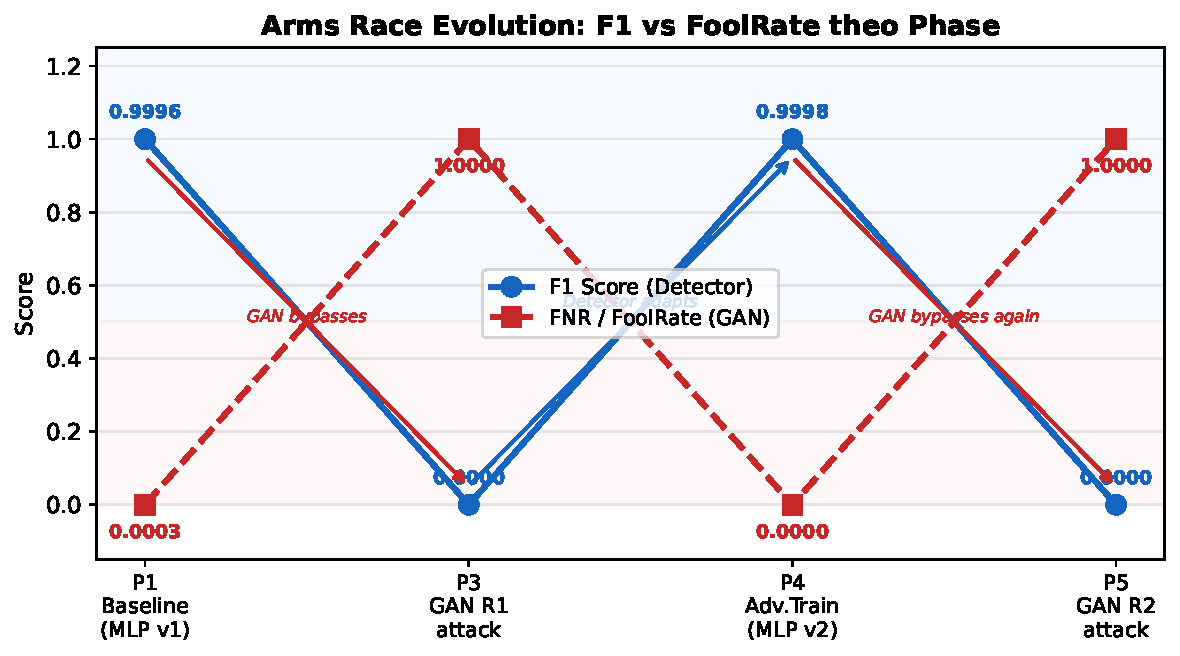
\includegraphics[width=0.82\textwidth,height=0.38\textheight,keepaspectratio]{fig_timeline}
  \end{center}
\end{frame}

\begin{frame}{Hướng B: FoolRate qua các Round}
  \begin{columns}[T]
    \begin{column}{0.58\textwidth}
      \begin{center}
        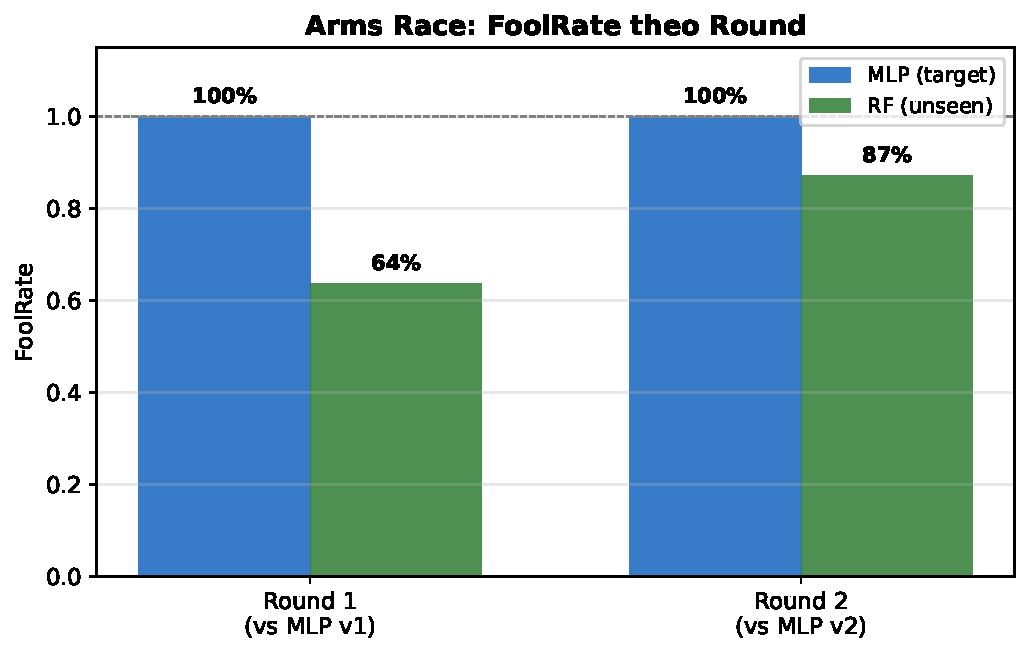
\includegraphics[width=\textwidth,height=0.72\textheight,keepaspectratio]{fig_armsrace}
      \end{center}
    \end{column}
    \begin{column}{0.39\textwidth}
      \begin{block}{Nhận xét}
        \begin{itemize}\setlength\itemsep{5pt}
          \item MLP FoolRate = \textbf{100\%} cả 2 rounds
          \item RF FoolRate tăng $63.7\%\! \to\! 87.2\%$\\ Transferability cải thiện
          \item GAN học patterns tổng quát hơn theo round
        \end{itemize}
      \end{block}
    \end{column}
  \end{columns}
\end{frame}

\begin{frame}{Hướng B: Transferability -- GAN bypass cross-architecture}
  \begin{columns}[T]
    \begin{column}{0.50\textwidth}
      \begin{block}{Thí nghiệm Transferability}
        GAN được train \textbf{chỉ} trên MLP Detector,\\ sau đó test trên \textbf{Random Forest} -- kiến trúc hoàn toàn khác
      \end{block}
      \vspace{6pt}
      \small
      \begin{tabular}{lccc}
        \toprule
        & \multicolumn{2}{c}{\textbf{FoolRate}} \\
        \cmidrule{2-3}
        \textbf{Detector} & \textbf{Round 1} & \textbf{Round 2} \\
        \midrule
        MLP v1 (target R1) & 1.0000 & 0.0008 \\
        MLP v2 (target R2) & --     & 1.0000 \\
        \textbf{RF (unseen)} & \textbf{0.6371} & \textbf{0.8716} \\
        \bottomrule
      \end{tabular}
    \end{column}
    \begin{column}{0.47\textwidth}
      \begin{alertblock}{Findings}
        \begin{itemize}\setlength\itemsep{4pt}
          \item RF FoolRate \textbf{tăng} từ $63.7\% \to 87.2\%$ (Round 1 $\to$ 2)
          \item GAN round 2 học được features tổng quát hơn khi phải bypass detector mạnh hơn
          \item \textbf{Rủi ro thực tế:} Adversarial samples có thể bypass nhiều loại IDS, không chỉ target
          \item GAN Round 2 chuyên biệt hóa: MLP v1 FoolRate giảm xuống 0.08\%
        \end{itemize}
      \end{alertblock}
    \end{column}
  \end{columns}
\end{frame}

\begin{frame}{Hướng B: KL Divergence --- Chất lượng phân phối}
  \begin{center}
    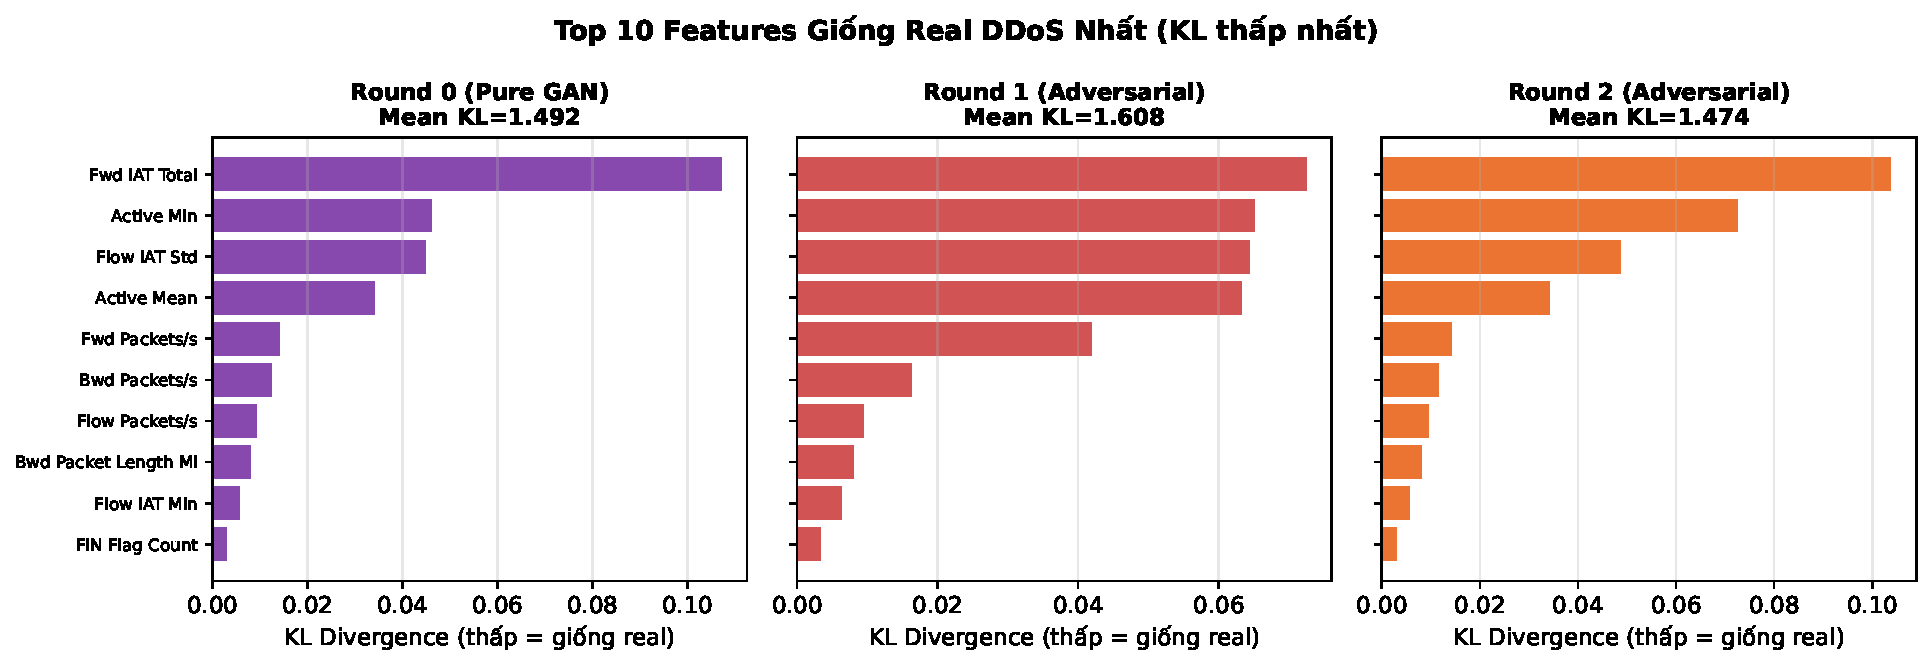
\includegraphics[width=0.97\textwidth,height=0.76\textheight,keepaspectratio]{fig_kl}
  \end{center}
  \vspace{-4pt}
  \centering\footnotesize
  Top 10 features giống real nhất (KL thấp nhất). Round 0 có Mean KL thấp hơn --- fake gần real DDoS hơn.
\end{frame}

\begin{frame}{SHAP: Giải thích thay đổi của Detector}
  \begin{columns}[T]
    \begin{column}{0.50\textwidth}
      \begin{block}{Mục tiêu SHAP}
        So sánh feature importance của Detector v1 vs v2 sau adversarial training:\\
        \textit{Liệu v2 có chú trọng hơn vào functional features?}
      \end{block}
      \vspace{6pt}
      \begin{tabular}{lccc}
        \toprule
        \textbf{Group} & \textbf{v1} & \textbf{v2} & $\mathbf{\Delta}$ \\
        \midrule
        Functional     & 0.4794 & 0.4458 & \textcolor{danger}{$-$0.034} \\
        Non-functional & 0.4660 & 0.3998 & \textcolor{danger}{$-$0.066} \\
        \bottomrule
      \end{tabular}
    \end{column}
    \begin{column}{0.47\textwidth}
      \begin{alertblock}{Finding}
        \begin{itemize}\setlength\itemsep{4pt}
          \item \textbf{Không có shift} từ non-functional sang functional features
          \item Cả hai group \textbf{giảm} sau adv. training -- model trở nên \textit{less confident} tổng thể
          \item GAN bypass qua \textbf{non-functional features} (consistent với Validity=0)
        \end{itemize}
      \end{alertblock}
      \vspace{4pt}
      \begin{exampleblock}{Implication}
        Để detector mạnh hơn, cần penalize GAN khi modify \textbf{functional features} -- đây là lý do cần constraint loss $\mathcal{L}_{con}$
      \end{exampleblock}
    \end{column}
  \end{columns}
\end{frame}

\begin{frame}{SHAP: Biểu đồ Feature Importance}
  \begin{columns}[T]
    \begin{column}{0.62\textwidth}
      \begin{center}
        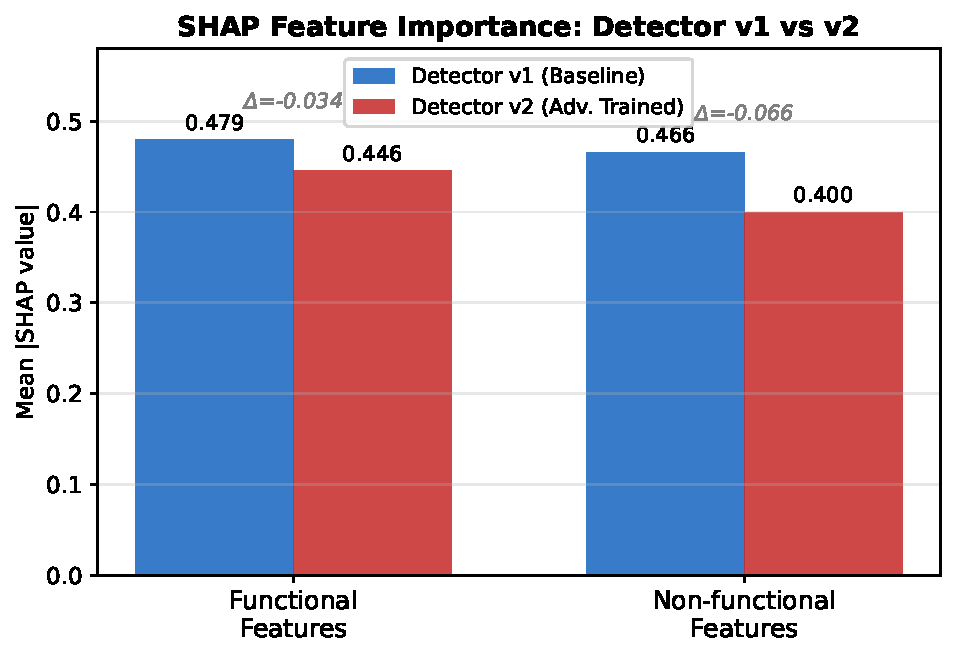
\includegraphics[width=\textwidth,height=0.72\textheight,keepaspectratio]{fig_shap}
      \end{center}
    \end{column}
    \begin{column}{0.35\textwidth}
      \begin{alertblock}{Finding}
        \begin{itemize}\setlength\itemsep{5pt}
          \item Cả hai group \textbf{giảm} sau adv. training
          \item Không có shift\\ non-func $\to$ functional
          \item Model \textit{less confident} tổng thể
        \end{itemize}
      \end{alertblock}
    \end{column}
  \end{columns}
\end{frame}

%% =============================================================================
\section{6. Kết luận}
%% =============================================================================

\begin{frame}{Tóm tắt kết quả}
  \begin{columns}[T]
    \begin{column}{0.50\textwidth}
      \begin{exampleblock}{Đã đạt được}
        \begin{itemize}\setlength\itemsep{4pt}
          \item[\YES] \textbf{Hướng A}: 5/16 functional features\\validity $>$ 99\% với $\lambda_c=5.0$
          \item[\YES] \textbf{Hướng B}: GAN bypass hoàn toàn\\cả Detector v1 \& v2 (F1 = 0.0)
          \item[\YES] \textbf{Adv. Training}: Detector v2 phục hồi\\(F1=0.9998 trên adversarial set)
          \item[\YES] \textbf{Transferability}: RF FoolRate $63.7\% \to 87.2\%$
          \item[\YES] \textbf{SHAP}: Phân tích attention shift
          \item[\YES] \textbf{Validity Score}: Metric mới đề xuất
        \end{itemize}
      \end{exampleblock}
    \end{column}
    \begin{column}{0.47\textwidth}
      \begin{alertblock}{Hạn chế \& Hướng phát triển}
        \begin{itemize}\setlength\itemsep{4pt}
          \item[\NO] Overall Validity = 0 do AND condition\\
                \small $\to$ Cần post-processing hoặc Conditional GAN
          \item[\NO] SHAP không thấy attention shift\\
                \small $\to$ Cần thêm epochs / stronger adv. training
          \item[\NO] Chỉ 1 dataset (CIC-DDoS2019)\\
                \small $\to$ Thêm UNSW-NB15, CICIDS2017
          \item[\NO] Chưa so sánh với FGSM, PGD\\
                \small $\to$ Cần baseline comparison cho paper
        \end{itemize}
      \end{alertblock}
    \end{column}
  \end{columns}
\end{frame}

\begin{frame}{Kết luận}
  \begin{block}{Pipeline hoàn chỉnh đã triển khai}
    \centering
    \small
    Data $\to$ \textcolor{detcolor}{\textbf{Detector v1}} $\xrightarrow{\text{bypass}}$
    \textcolor{gancolor}{\textbf{GAN Round 1}} $\xrightarrow{\text{adv. train}}$
    \textcolor{detcolor}{\textbf{Detector v2}} $\xrightarrow{\text{bypass}}$
    \textcolor{gancolor}{\textbf{GAN Round 2}}
  \end{block}

  \vspace{10pt}
  \begin{itemize}\setlength\itemsep{6pt}
    \item \textbf{Đề tài hoàn thành:} Pipeline sinh mẫu DDoS bằng GAN kết hợp arms race với detector
    \item \textbf{Finding chính:} GAN bypass hoàn toàn MLP detector (F1: $0.9996 \to 0.0000$); Transferability cross-architecture đạt \textbf{87.2\%}
    \item \textbf{Validity Score:} Metric mới -- chưa có paper nào áp dụng trên CIC-DDoS2019
    \item \textbf{Hướng tiếp theo:} Conditional GAN + constraint mạnh hơn để tăng Validity $> 0$ toàn bộ
  \end{itemize}
\end{frame}

\begin{frame}[plain]
  \vfill
  \centering
  \textbf{\LARGE THANK YOU!}
  \vfill
\end{frame}

\end{document}
